\begin{appendixes}
    \section{Ap\'endice A: Soluci\'on de la ecuaci\'on de crecimiento log\'istico sujeta a las condiciones iniciales}
    \label{app-a}
    
    \begin{equation*}
    \boxed{\left\lbrace
        \begin{array}{l}		
            \displaystyle\frac{dP}{dt} = rP(1-\displaystyle\frac{P}{K})\\
            P(t=0)=P_0
        \end{array}
    \right.}
    \end{equation*}
    
    \begin{minipage}[t]{0.45\textwidth}
    \begin{enumerate}
    \item [(1.)] $\displaystyle \frac{dP}{dt} = rP(1-\frac{P}{K})$
    \item [(2.)] $\displaystyle rdt = \frac{dP}{P(1-\frac{P}{K})}$
    \item [(3.)] $\displaystyle \int rdt = \int \frac{dP}{P(1-\frac{P}{K})}$
    \item [(4.)] $\displaystyle \int rdt = \int \frac{1}{P}dP + \int \frac{\frac{1}{K}}{1-\frac{P}{K}}dP \\ *(\displaystyle u=1-\frac{P}{K},~\displaystyle du=-\frac{1}{K}dP)$
    \item [(5.)] $\displaystyle rt+C = \ln P - \ln(1-\frac{P}{K})$
    \item [(6.)] $\displaystyle e^{rt+C} = e^{lnP - \ln(1-\frac{P}{K})}$
    \item [(7.)] $\displaystyle e^{rt+C} = \frac{e^{\ln P}}{e^{\ln(1-\frac{P}{K})}}$
    \end{enumerate}
    \end{minipage} \hfill 
    \begin{minipage}[t]{0.45\textwidth}
    \begin{enumerate}
    \item [(8.)] $\displaystyle e^{rt}e^C = \frac{P}{1-\frac{P}{K}}$
    \item [(9.)] $\displaystyle Ae^{rt} = \frac{P}{1-\frac{P}{K}}$
    \item [(10.)] $\displaystyle P = \frac{AK}{Ke^{-rt}+A} \\ *(P(t=0)=P_0)$
    \item [(11.)] $\displaystyle P_0 = \frac{AK}{K+A}$
    \item [(12.)] $\displaystyle A = \frac{K P_0}{K-P_0}$
    \item [(13.)] $\displaystyle P = \frac{\frac{K P_0}{K-P_0}K}{Ke^{-rt}+\frac{K P_0}{K-P_0}}$
    \end{enumerate}
    \end{minipage}
    
    \begin{equation*}
    \boxed{P(t) = \displaystyle\frac{P_0 K}{P_0 + (K-P_0)e^{-rt}}}
    \end{equation*}
    
    \section{Ap\'endice B: Derivaci\'on de la funci\'on P(t) para su utilizaci\'on como funci\'on de probabilidad}
    \label{app-b}
    
    \begin{equation*}
    \boxed{P(t) = \displaystyle\frac{P_0 K}{P_0 + (K-P_0)e^{-rt}}}
    \end{equation*}
    
    \begin{enumerate}
    \item [(1.)] $P'(t) = \left[\displaystyle\frac{P_0 K}{P_0 + (K-P_0)e^{-rt}}\right]'$
    \item [(2.)] $f = P_0 K $
    \item [(3.)] $f' = (P_0 K)' = 0$
    \item [(4.)] $g = P_0 + (K-P_0)e^{-rt} = P_0 + K e^{-rt} - P_0 e^{-rt}$
    \item [(5.)] $g' = (P_0 + (K-P_0)e^{-rt})' = (P_0 + K e^{-rt} - P_0 e^{-rt})' = P_0 r e^{-rt} - K r e^{-rt}$
    \item [(6.)] $g^2 = (P_0 + (K-P_0)e^{-rt})^2 = (P_0 + K e^{-rt} - P_0 e^{-rt})^2$
    \item [(7.)] $P'(t) = \displaystyle\frac{P_0 K(K r e^{-rt} - P_0 r e^{-rt})}{(P_0 + K e^{-rt} - P_0 e^{-rt})^2}$
    \item [(8.)] $P'(t) = \displaystyle\frac{P_0 K(r e^{-rt}(K - P_0))}{(P_0 + K e^{-rt} - P_0 e^{-rt})^2}$
    \item [(9.)] $P'(t) = \displaystyle\frac{P_0 K r e^{-rt}(K - P_0)}{(P_0 + K e^{-rt} - P_0 e^{-rt})^2} \cdot \displaystyle\frac{e^{2rt}}{e^{2rt}}$
    \item [(10.)] $P'(t) = \displaystyle\frac{P_0 K r e^{rt}(K - P_0)}{(P_0 e^{rt} - P_0 + K)^2}$
    \end{enumerate}
    
    \begin{equation*}
    \boxed{P'(t) = \displaystyle\frac{P_0 K r e^{rt}(K-P_0)}{(P_0 e^{rt} - P_0 + K)^2}}
    \end{equation*}
    
    \section{Ap\'endice C: Derivaci\'on de la funci\'on P'(t) para la b\'usqueda de sus puntos estacionarios}
    \label{app-c}
    
    \begin{equation*}
    \boxed{P'(t) = \displaystyle\frac{P_0 K r e^{rt}(K-P_0)}{(P_0 e^{rt} - P_0 + K)^2}}
    \end{equation*}
    
    \begin{enumerate}
    \item [(1.)] $P''(t) = \left[\displaystyle\frac{P_0 K r e^{rt}(K-P_0)}{(P_0 e^{rt} - P_0 + K)^2}\right]'$
    \item [(2.)] $f = P_0 K r e^{rt}(K-P_0) = P_0 K^2 r e^{rt} - P_0 K r e^{rt}$
    \item [(3.)] $f' = (P_0 K r e^{rt}(K-P_0))' = P_0 K r^2 e^{rt}(K-P_0) = P_0 K^2 r^2 e^{rt} - P_0 K r^2 e^{rt}$
    \item [(4.)] $g = (P_0 e^{rt} - P_0 + K)^2 = P_0^2 e^{2rt} - 2P_0^2 e^{rt} + 2P_0 K e^{rt} - 2P_0 K + P_0^2 + K^2$
    \item [(5.)] $g' = ((P_0 e^{rt} - P_0 + K)^2)' = 2P_0^2 r e^{2rt} - 2P_0^2 r e^{rt} + 2P_0 K r e^{rt}$
    \item [(6.)] $g^2 = ((P_0 e^{rt} - P_0 + K)^2)^2 = (P_0 e^{rt} - P_0 + K)^4$
    \item [(7.)] $P''(t) = \displaystyle\frac{3P_0^3 K^2 r^2 e^{rt} + P_0 K^4 r^2 e^{rt} + P_0^4 K r^2 e^{3rt} - 3P_0^2 K^3 r^2 e^{rt} - P_0^3 K^2 r^2 e^{3rt} - P_0^4 K r^2 e^{rt}}{(P_0e^{rt} - P_0 + K)^4}$
    \item [(8.)] $P''(t) = \displaystyle\frac{P_0^3 K r^2 e^{3rt}(P_0-K) + 3P_0^2 K^2 r^2 e^{rt}(P_0-K) - P_0 K r^2 e^{rt}(P_0^3 - K^3)}{(P_0e^{rt} - P_0 + K)^4}$
    \item [(9.)] $P''(t) = \displaystyle\frac{(P_0-K)(P_0^3 K r^2 e^{3rt} + 2P_0^2 K^2 r^2 e^{rt} - P_0 K^3 r^2 e^{rt} - P_0^3 K r^2 e^{rt})}{(P_0e^{rt} - P_0 + K)^4}$
    \item [(10.)] $P''(t) = \displaystyle\frac{P_0 K r^2 e^{rt}(P_0-K)(P_0^2 e^{2rt} + 2P_0 K - K^2 - P_0^2)}{(P_0e^{rt} - P_0 + K)^4}$
    \item [(11.)] $P''(t) = \displaystyle\frac{P_0 K r^2 e^{rt}(P_0-K)(P_0 e^{rt} + P_0 - K)(P_0 e^{rt} - P_0 + K)}{(P_0e^{rt} - P_0 + K)^4}$
    \item [(12.)] $P''(t) = \displaystyle\frac{P_0 K r^2 e^{rt}(P_0-K)(P_0 e^{rt} + P_0 - K)}{(P_0 e^{rt} - P_0 + K)^3}$
    \item [(13.)] $0 = e^{rt}(P_0-K)(P_0 e^{rt} + P_0 - K)$
    \item [(14.)] $0 = P_0 e^{rt} + P_0 - K$
    \item [(15.)] $e^{rt} = \displaystyle\frac{K-P_0}{P_0}$
    \item [(16.)] $\ln e^{rt} = \ln \displaystyle\frac{K-P_0}{P_0}$
    \item [(17.)] $rt = \ln \displaystyle\frac{K-P_0}{P_0}$
    \item [(18.)] $t = \displaystyle\frac{1}{r} \ln \frac{K-P_0}{P_0} $
    \end{enumerate}
    
    \begin{align*}
    \boxed{P''(t) = \displaystyle\frac{P_0 K r^2 e^{rt} (P_0-K)(P_0 e^{rt} + P_0 - K)}{(P_0 e^{rt} - P_0 + K)^3}} \quad \boxed{t = \displaystyle\frac{1}{r} \ln \displaystyle\frac{K-P_0}{P_0}}
    \end{align*}
    
    \section{Ap\'endice D: Diversos tipos de epitelios del organismo}
    \label{app-d}
    
    \begin{description}
    \item [Escamoso simple] -- Se encuentra en los alv\'eolos pulmonares y como recubrimiento de las cavidades del coraz\'on y de los vasos sangu\'ineos y linf\'aticos. Presenta una \'unica capa de c\'elulas de un grosor total aproximado de $0$.$02mm$.
    
    \item [C\'ubico simple] -- Se encuentra en los ductos de gl\'andulas secretoras como la tiroides, y en los t\'ubulos del ri\~non. Presenta una \'unica capa de c\'elulas de un grosor total aproximado de $0$.$035mm$.
    
    \item [Columnar simple] -- Se encuentra en los bronquios, \'utero, tracto digestivo y vejiga. Presenta una \'unica capa de c\'elulas de un grosor total aproximado de $0$.$1mm$.
    
    \item [Columnar pseudoestratificado] -- Se encuentra en la tr\'aquea, en la mayor\'ia del tracto respiratorio superior y en los conductos auditivos. Presenta una \'unica capa de c\'elulas de un grosor total aproximado de $0$.$1mm$.
    
    \item [Columnar estratificado] -- Se encuentra principalmente en la uretra, faringe y en los ductos de algunas gl\'andulas. Presenta dos capas de c\'elulas de un grosor total aproximado de $0$.$1mm$.
    
    \item [C\'ubico estratificado] -- Se encuentra en las gl\'andulas sudor\'iparas, salivares y mamarias. Presenta dos capas de c\'elulas de un grosor total aproximado de $0$.$05mm$.
    
    \item [Escamoso estratificado] -- Se encuentra como recubrimiento del es\'ofago, boca y vagina. Presenta de cuatro a cinco capas de c\'elulas de un grosor total aproximado de $0$.$06mm$.
    
    \item [Transicional] -- Se encuentra en el interior de la vejiga y la uretra. Presenta de tres a cinco capas de c\'elulas de un grosor total aproximado de $0$.$07mm$.
    \end{description}
    
    \begin{figure}[!ht]
    \begin{center}
    \scalebox{0.6}{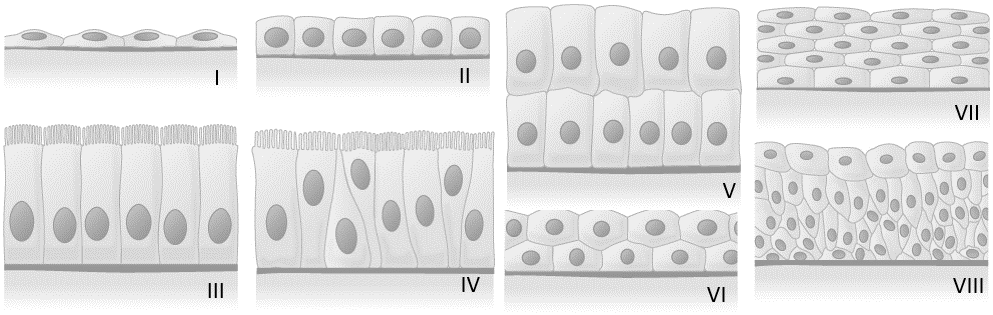
\includegraphics{img/fig-epitheliums.png}}
    \end{center}
    \caption[Diagramas mostrando los distintos tipos de epitelios del organismo]{Diagramas mostrando los distintos tipos de epitelios del organismo: escamoso simple~(\emph{I});  c\'ubico simple~(\emph{II}); columnar simple~(\emph{III}); columnar pseudoestratificado~(\emph{IV}); columnar estratificado~(\emph{V}); c\'ubico estratificado~(\emph{VI}); escamoso estratificado~(\emph{VII}); y transicional~(\emph{VIII}). (Figura tomada de~\cite{robins}).}
    \label{fig-epitheliums}
    \end{figure}
    
    \section{Ap\'endice E: Simulaci\'on del ciclo vital del c\'ancer para un tumor primario con un alto potencial metast\'asico en el interior de un ducto mamario}
    \label{app-e}
    
    \begin{table}[!ht]
    \begin{center}
    \scalebox{0.9}{\begin{tabular}{|p{2.5cm}|p{14cm}|}\hline
        \emph{Red} & $s_x=200$; $s_y=100$; $s_z=100$; $s_o=100$; $p = 0$.$01$. \\\hline
    
    \emph{Estados} & Para el \'organo primario correspondiente con la mama -- Esquema I: $v_x^t=50$, $v_y^t=50$, $v_z^t=50$. Para el \'organo secundario correspondiente con el pulm\'on -- Esquema I: $o_s=100$.\\\hline 
    
    \emph{Nutrientes} & Para el \'organo primario -- $R_1 = \lbrace v~|~v \in V(G) : (0 \leq v_x < 100) \wedge (0 \leq v_y < 50) \wedge (0 \leq v_z < 50) \rbrace$, $B_{01}=\lbrace \overrightarrow{\nu_{((0,0),(0,1))}} \rbrace$, $R_2 = \lbrace v~|~v \in V(G) : (0 \leq v_x < 100) \wedge (50 \leq v_y < 100) \wedge (50 \leq v_z < 100) \rbrace$. Para el \'organo secundario -- $R_3 = \lbrace v~|~v \in V(G) : (100 \leq v_x < 200) \wedge (0 \leq v_y < 100) \wedge (0 \leq v_z < 100) \rbrace$.\\\hline
    
    \emph{Crecimiento} & Avascular -- $P_0^a=1$, $K_a=2$.$222 \times 10^2$, $r_a=1$.$802 \times 10^{-2}$, $\Delta t=2$.$996 \times 10^1$, $n_a=20$, generaciones del aut\'omata: $21$~($63$ d\'ias). Vascular -- $P_0^v=2$.$222 \times 10^2$, $K_v=5$.$556 \times 10^4$, $r_v=7$.$199 \times 10^{-5}$, $\Delta t=7$.$665 \times 10^2$, generaciones del aut\'omata: $321$~($963$ d\'ias).\\\hline
    
    \emph{Migraci\'on} & Aparici\'on de c\'elulas migratorias -- $\eta_{mig}=1$, $K_{mig}=5$.$0 \times 10^5$, probabilidad de aparici\'on $0$.$1$. Movilidad -- $\mu_{mig}=1$, $\eta_{mig}'=0$.$1$, $\mu_{max}=100$.\\\hline
    
    \emph{Met\'astasis} & Huesos -- $\xi_{mic} = 0$.$981$, $\psi_{mic} = 6$.$0 \times 10^{-4}$. Mama -- $\xi_{mic} = 0$.$9571$, $\psi_{mic} = 1$.$0 \times 10^{-4}$; $\xi_{sc} = 5$.$0 \times 10^{-4}$. \\\hline
    \end{tabular}}
    \end{center}\vspace*{-0.6cm}
    \caption[Ap\'endice E: par\'ametros de la simulaci\'on]{Par\'ametros de la simulaci\'on.}
    \end{table}
    
    \begin{figure}[!ht]
    \begin{center}
        \subfigure[Generaci\'on 4]{\scalebox{0.29}{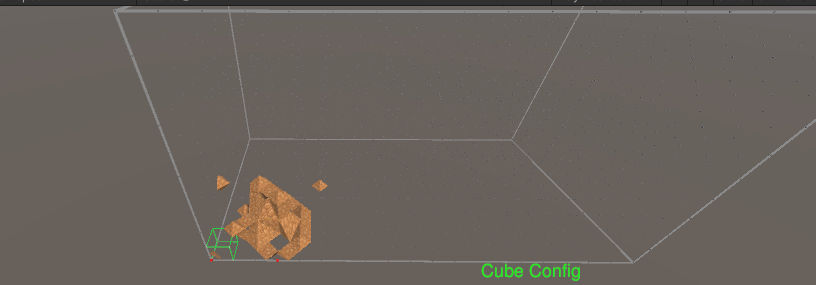
\includegraphics{img/automata/apendix/1.png}}}
        \subfigure[Generaci\'on 30]{\scalebox{0.29}{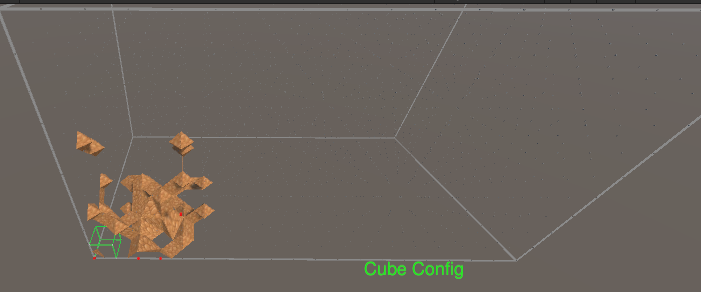
\includegraphics{img/automata/apendix/2.png}}}
        \subfigure[Generaci\'on 45]{\scalebox{0.29}{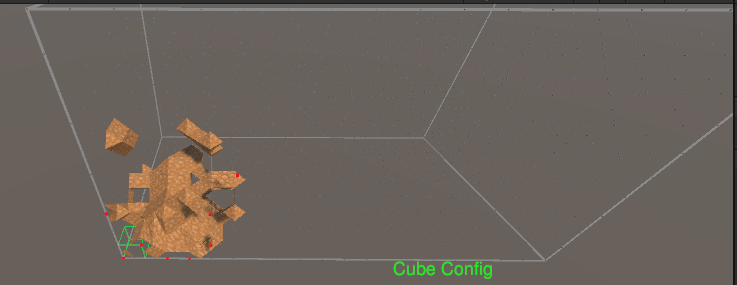
\includegraphics{img/automata/apendix/3.png}}}
    \subfigure[Generaci\'on 70]{\scalebox{0.29}{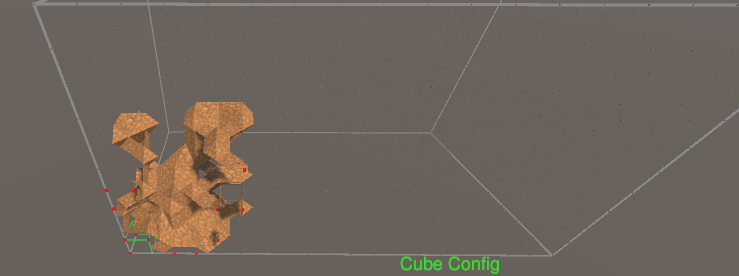
\includegraphics{img/automata/apendix/4.png}}}
    % \subfigure[Generaci\'on 16]{\scalebox{0.29}{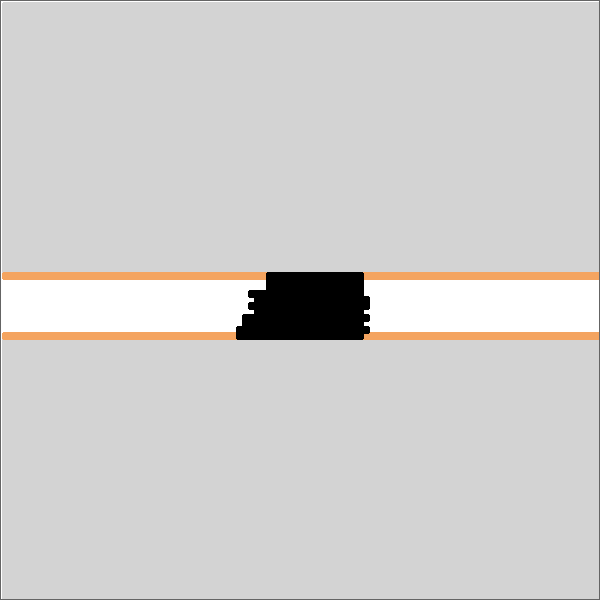
\includegraphics{img/automata/apendix/16-201952918297-Primary.png}}}
    % \subfigure[Generaci\'on 20]{\scalebox{0.29}{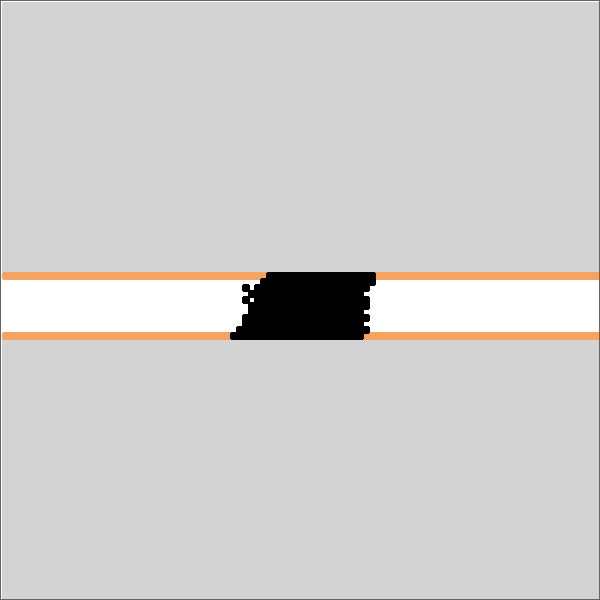
\includegraphics{img/automata/apendix/20-201952918297-Primary.png}}}
    \end{center}\vspace*{-0.75cm}
    \caption[Ap\'endice E: visualizaciones de la simulaci\'on del aut\'omata celular durante la etapa avascular]{Ap\'endice E: visualizaciones de la simulaci\'on del aut\'omata celular durante la etapa avascular. El \'area mostrada posee dimensiones $[0,10$.$5]mm \times [0,10$.$5]mm \times [0,10$.$5]mm$.}
    \end{figure}
    
    \begin{figure}[!ht]
    \begin{center}
        \subfigure[Generaci\'on 150]{\scalebox{0.23}{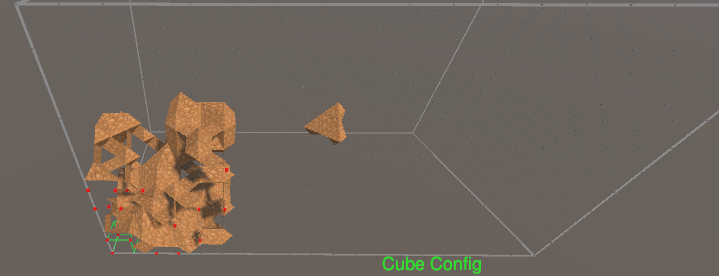
\includegraphics{img/automata/apendix/5.png}}}
    
    % \scalebox{0.23}{
\includegraphics{img/automata/apendix/99-201952918297-Secondary.png}}}
    \subfigure[Generaci\'on 175]{\scalebox{0.23}{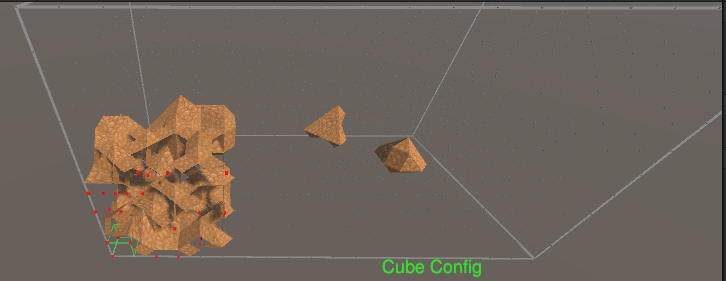
\includegraphics{img/automata/apendix/6.png}}}
    \subfigure[Generaci\'on 200]{\scalebox{0.23}{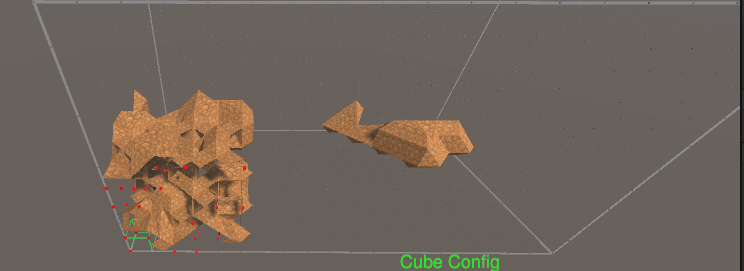
\includegraphics{img/automata/apendix/7.png}}}
    
    % \subfigure[Generaci\'on 165]{\scalebox{0.23}{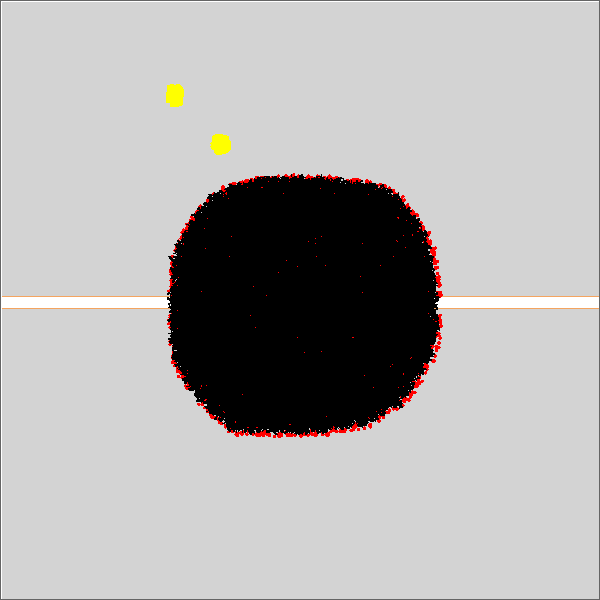
\includegraphics{img/automata/apendix/165-201952918297-Primary.png}}
    % \scalebox{0.23}{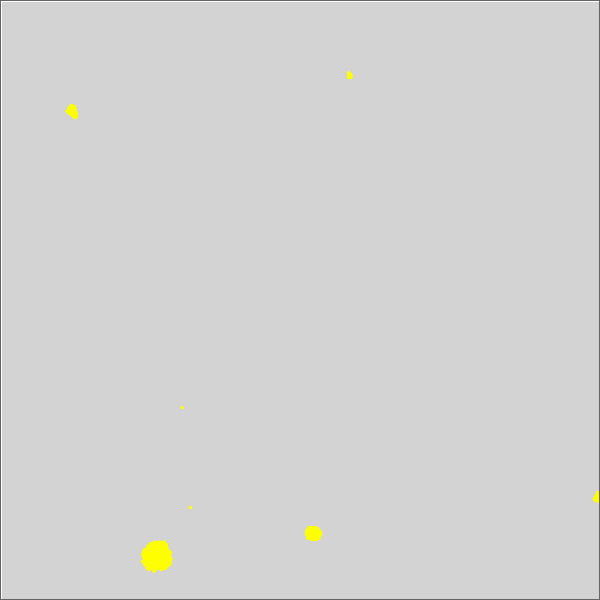
\includegraphics{img/automata/apendix/165-201952918297-Secondary.png}}}
    % \subfigure[Generaci\'on 198]{\scalebox{0.23}{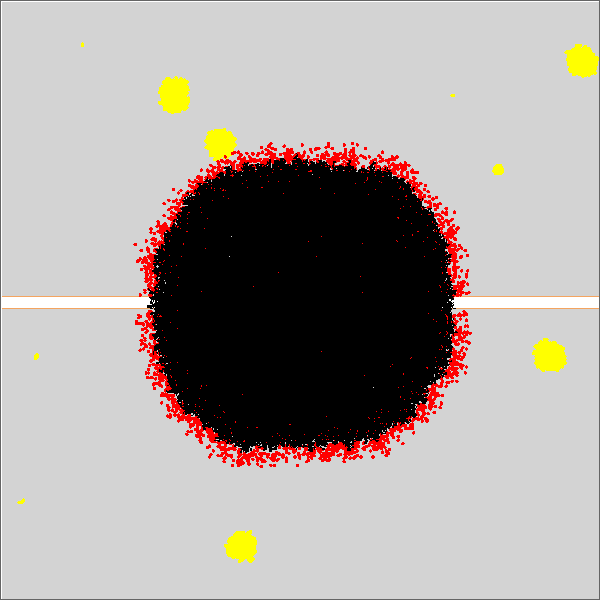
\includegraphics{img/automata/apendix/198-201952918297-Primary.png}}
    % \scalebox{0.23}{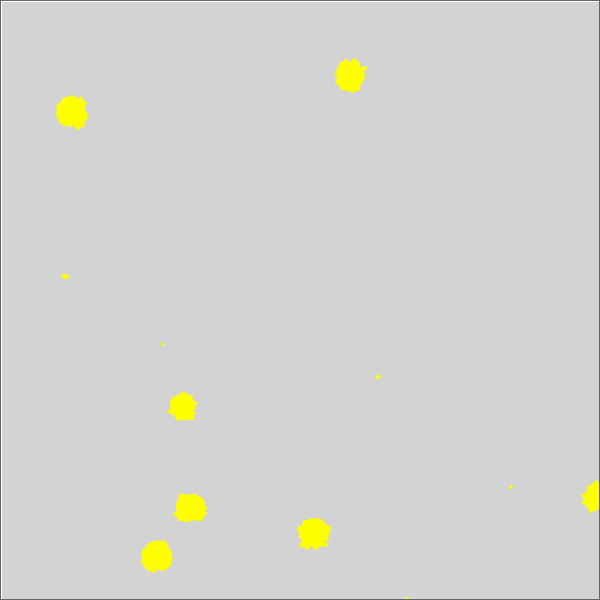
\includegraphics{img/automata/apendix/198-201952918297-Secondary.png}}}\vspace*{-0.2cm}
    
    % \subfigure[Generaci\'on 231]{\scalebox{0.23}{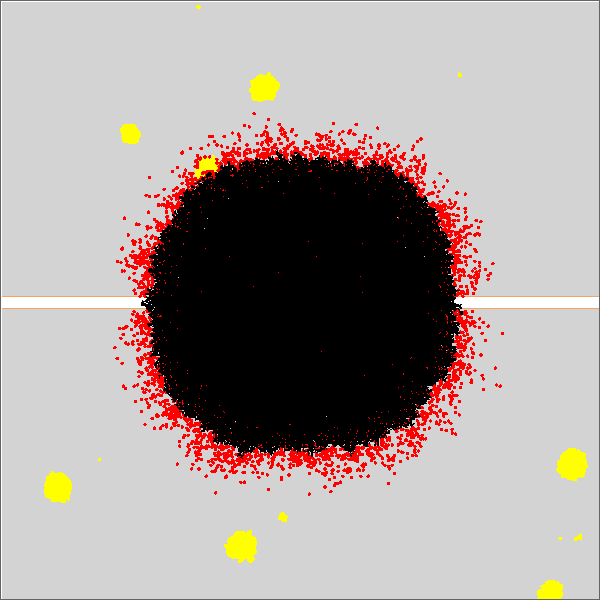
\includegraphics{img/automata/apendix/231-201952918297-Primary.png}}
    % \scalebox{0.23}{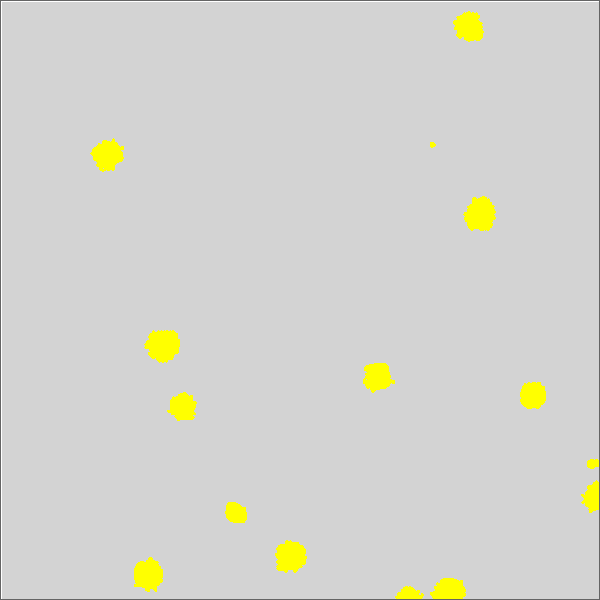
\includegraphics{img/automata/apendix/231-201952918297-Secondary.png}}}
    % \subfigure[Generaci\'on 264]{\scalebox{0.23}{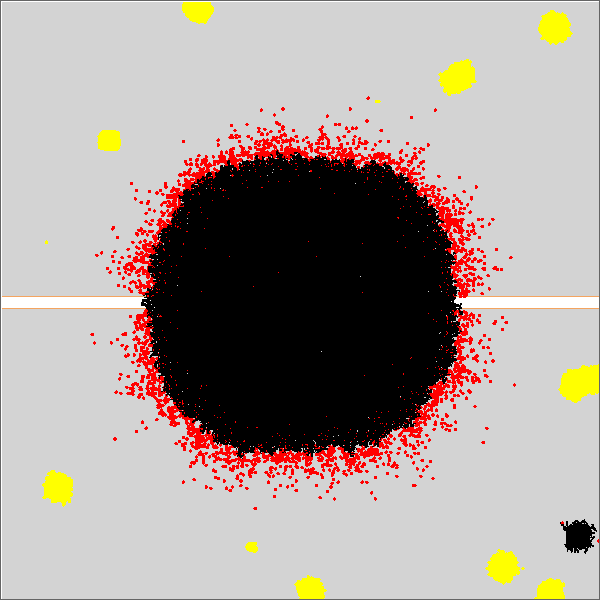
\includegraphics{img/automata/apendix/264-201952918297-Primary.png}}
    % \scalebox{0.23}{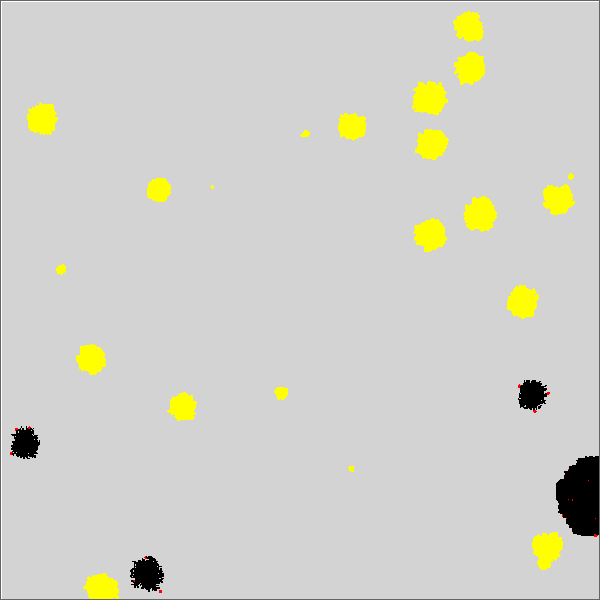
\includegraphics{img/automata/apendix/264-201952918297-Secondary.png}}}\vspace*{-0.2cm}
    
    % \subfigure[Generaci\'on 297]{\scalebox{0.23}{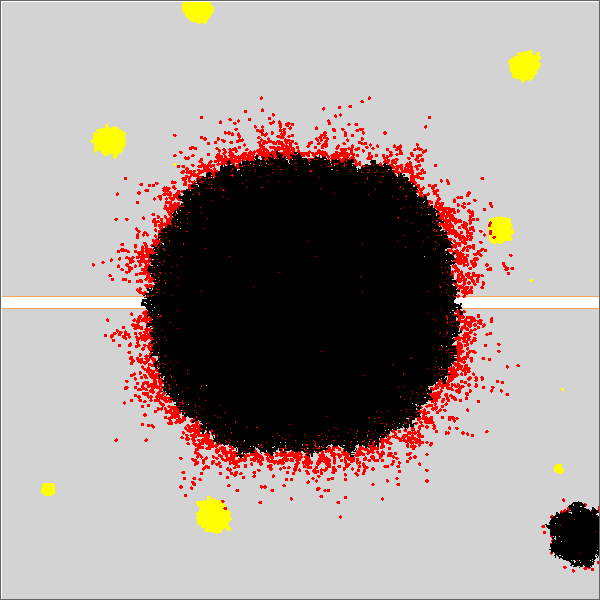
\includegraphics{img/automata/apendix/297-201952918297-Primary.png}}
    % \scalebox{0.23}{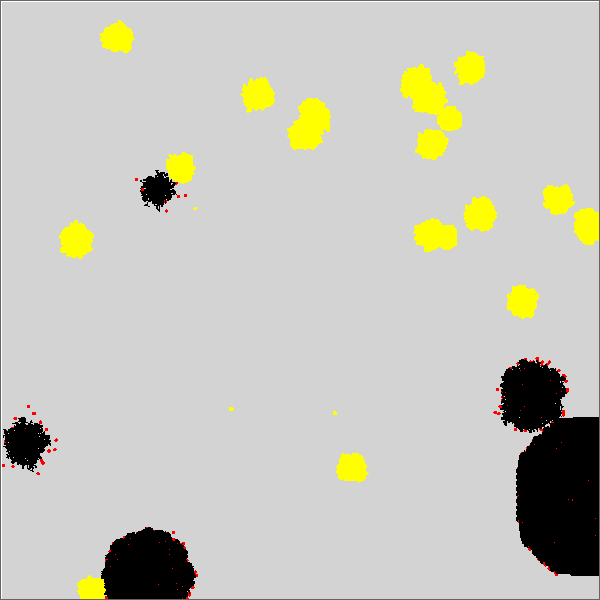
\includegraphics{img/automata/apendix/297-201952918297-Secondary.png}}}
    % \subfigure[Generaci\'on 321]{\scalebox{0.23}{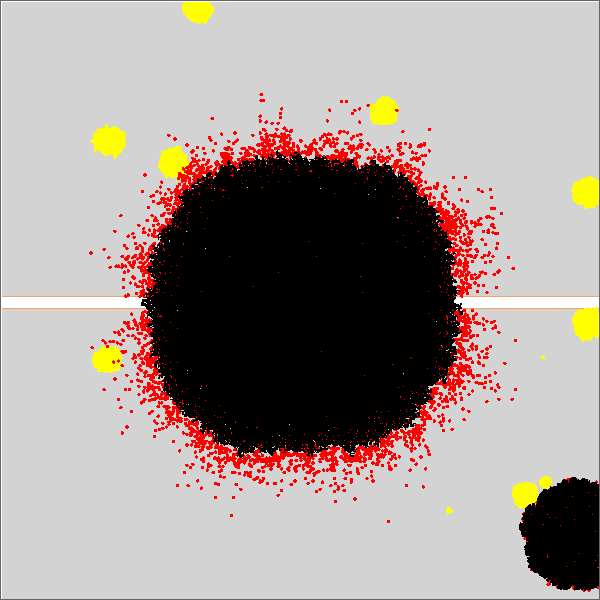
\includegraphics{img/automata/apendix/321-201952918297-Primary.png}}
    % \scalebox{0.23}{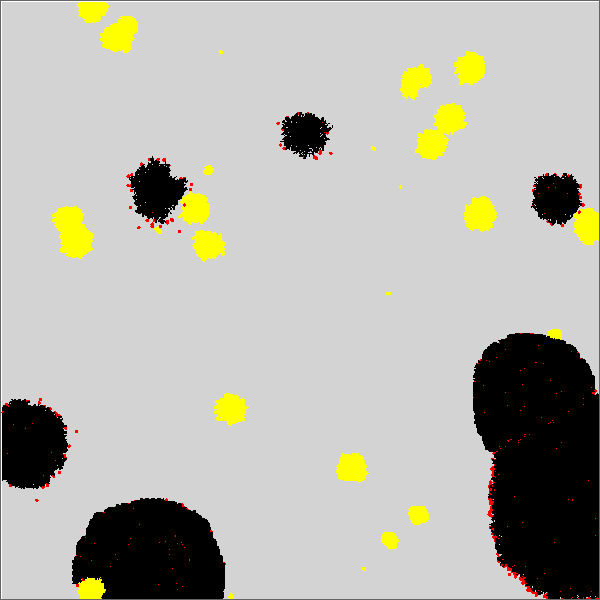
\includegraphics{img/automata/apendix/321-201952918297-Secondary.png}}}\vspace*{-0.2cm}
    \end{center}\vspace*{-0.6cm}
    \caption[Ap\'endice E: visualizaciones de la simulaci\'on del aut\'omata celular durante la etapa vascular]{Ap\'endice E: visualizaciones de la simulaci\'on del aut\'omata celular durante la etapa vascular. El tumor de mayor \'area es el principal y el de menor \'area es el secundario que est\'a llevando a cabo la met\'astasis. El \'area mostrada para cada localizaci\'on posee dimensiones $[0,52$.$5]mm \times [0,52$.$5]mm \times [0,52$.$5]mm$.}
    \end{figure}
\end{appendixes}